\documentclass[letterpaper]{article}
\title{Auto Scaling for Analytics on Streaming Data}
\date{}
\usepackage{balance}  % to better equalize the last page
\usepackage{graphicx}
\usepackage{times}    % comment if you want LaTeX's default font
\usepackage{url}      % llt: nicely formatted URLs
\usepackage{graphicx}
\usepackage{tabularx}
\usepackage{float}
\usepackage{color}
\usepackage{url}
\usepackage[noend]{algpseudocode}
\usepackage{algorithm}
\usepackage{verbatim}
\usepackage{mathtools}
\usepackage{caption}
\usepackage{subcaption}
%\usepackage{amsmath}
\let\proof\relax
\let\endproof\relax
\usepackage{amsthm}
\usepackage{thmtools}
\usepackage{xspace}
\usepackage{multirow}
\newcommand{\field}[1]{\mathbb{#1}} 
\newcommand{\hide}[1]{#1}
\newcommand{\pd}[2]{\frac{\partial #1}{\partial #2}}
\providecommand{\m}[1]{\mathbf{#1}}
\providecommand{\norm}[1]{\left\|#1\right\|}
\providecommand{\sign}[1]{\text{sign}\left(#1\right)}
\DeclareMathOperator*{\argmin}{arg\,min}
\providecommand{\what}{\m{\hat{w}}}

\begin{document}
\author{CSE 550 Project Proposal \\\\ Marco Tulio Correia Ribeiro, Shrainik Jain\\ 1323300, 1323338}
\maketitle

\section{Background and Prior work}
The task of predicting the appropriate content to a user in an internet setting involves the concept of streaming data. A generic machine learning problem can be broken down into 2 major steps, 1 - Learning a model from data, and 2 - Making predictions according to the model. In case of streaming data, we need to constantly learn and update our model as we get newer data. There are multiple challenges while proposing a solution to this problem. \\First challenge is that the amount of data is always growing, so we cannot keep archiving it, both becuase of storage constraints and computation constraints. The usual solution to deal with this problem is to keep only the meaningful things about data, maybe just the model, and forget the rest of it, and when newer data comes in, use the newer data plus the existing model to come up with a newer model. This can be achieved by implementing incremental algorithms or with periodic re-training of the model with a batch algorithm. \\Second challenge is the velocity of this data. Imagine a learning problem where in the learning dataset is a live twitter stream for a hashtag. In this scenario the rate at which the data comes in is a function of the popularity of the hashtag. \\
The problem we are trying to solve is to automatically handle the changing storage and computions needs for such scenario by integrating intelligent scaling into the solution. Most of the current auto-scaling is implemented for services that are easily replicated. Some examples include the amazon web services which have an option for auto-scaling, but that entails just spawing a new server with the same app or the Google AppEngine, which scales approriately depending on the number of user requests. The assumption of easy replication is not true for machine learning scenarios.
\section{Proposed work}
We want implement some intelligent auto scaling while maintain the prediction service SOA, and some measurement of learning, with the minimum cost possible. This problem is difficult becuase we can't just spawn another instance, because learning in parallel is hard. One possible solution is to have one node always be the learners and scale the number of predictors. We also need some sort of a load balancer and a manager to decide when to set up more machines. These are non trivial problems as having a single learner or a single load balancer add single points of failure to the system and also limit scalablity. \\
The focus of this project won't be deal with the machine learning aspect, we plan to use some out-of-box tools for it, what we want to target on is:
\begin{itemize}
\item Determining when to start more machines.
\item What role the new machines should play.
\item When to shutdown some machines.
\item How to ensure the system is fault taulerant.
\end{itemize}
\section{Roadmap}
Project Milestone: 
\begin{itemize} 
\item This is a fairly new problem and we would devote some initial time towards looking at existing similar solutions and formalizing the problem we are trying to solve.
\item Propose an initial design for the auto scaling service.
\end{itemize}
Short Presentation:
\begin{itemize} 
\item Next step would be to set up (possibly simulated) environment and implement our auto scaling system using standard BigML tools. 
\end{itemize}
Final Report:
\begin{itemize}
\item Detailed design specifications. 
\item Learning and results from the implementation (possibly simulated)
\end{itemize}

\section{References}
%\begin{figure}[h!]
%\centering
%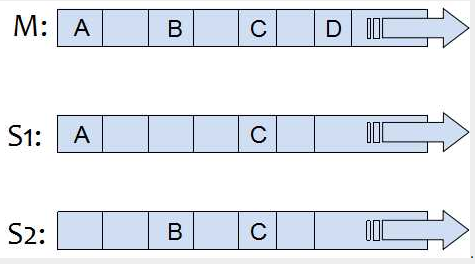
\includegraphics[scale=.5]{multipaxos.png}
%\caption{Illustration of multi-instance leader paxos. Source: StackOverflow.}
%\end{figure}

\end{document}
